\documentclass[a4paper,10pt,oneside]{book}
\usepackage{CS_report}
\usepackage[T1]{fontenc}
\usepackage{pifont}

\makeatletter
\pretocmd{\tableofcontents}{\hypersetup{linkcolor=black}}{}{}
\makeatother
\captionsetup[figure]{margin=1.5cm,font=small,name={Gambar},labelsep=colon}
\captionsetup[table]{margin=1.5cm,font=small,name={Tabel},labelsep=colon}

\begin{document}

    \frontmatter

    \begin{titlepage}
        \begin{center}

            \vspace{3cm}
            {\LARGE \textbf{Laporan Tugas Besar 2}}\\[0.5cm]
            {\Large IF2211 \textsc{Strategi Algoritma}}\\[0.2cm]
            {\large Pemanfaatan Algoritma BFS dan DFS dalam Mekanisme\\Penelusuran CSS pada Pohon Document Object Model}\\[0.2cm]
            {\normalsize Semester II Tahun 2025/2026}\\[1.5cm]

            \begin{figure}[htbp]
                \centering
                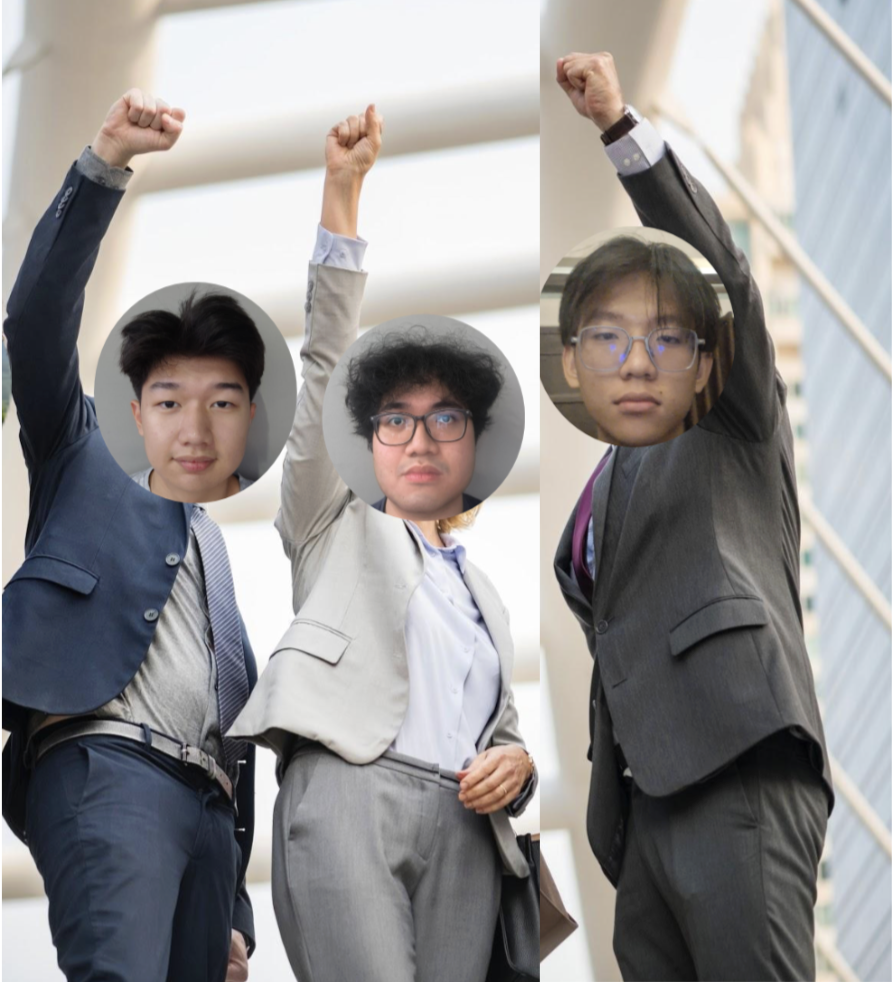
\includegraphics[width=8cm]{figures/kelompok.jpg}
                \label{fig:foto_kelompok}
            \end{figure}

            \vspace{1cm}

            \large Kelompok highAlcohol\\[0.5cm]

            \begin{tabular}{c}
                \Large{Stevanus Agustaf Wongso} \\ \Large{13524020} \\[0.3cm]
                \Large{Jonathan Kris Wicaksono} \\ \Large{13524023} \\[0.3cm]
                \Large{Philipp Hamara} \\ \Large{13524101} \\
            \end{tabular}

            \vspace{2cm}

            {\normalsize
            Laboratorium Ilmu dan Rekayasa Komputasi\\
            Program Studi Teknik Informatika\\
            Sekolah Teknik Elektro dan Informatika\\
            Institut Teknologi Bandung}\\[0.3cm]

        \end{center}
    \end{titlepage}

    \tableofcontents

    \mainmatter
    \chapter{Deskripsi Tugas}

\section{Latar Belakang}

\textit{Document Object Model} (DOM) adalah representasi terstruktur dari sebuah dokumen HTML dalam bentuk pohon yang memungkinkan setiap elemen pada halaman web untuk diakses, dimodifikasi, dan dimanipulasi secara terprogram. Struktur ini merepresentasikan relasi antar elemen HTML (\textit{parent}, \textit{child}, dan \textit{sibling}) sehingga sangat memudahkan pengolahan dokumen secara otomatis. Elemen \texttt{<html>} berperan sebagai \textit{root} yang membawahi dua bagian utama, yaitu \texttt{<head>} dan \texttt{<body>}.

Visualisasi dari pohon DOM dideklarasikan melalui \textit{Cascading Style Sheets} (CSS). Untuk mentargetkan elemen yang akan diberi gaya, CSS menggunakan mekanisme \textit{CSS Selector}. Mekanisme pencocokan selector terhadap pohon DOM pada dasarnya adalah proses \textit{graph traversal} terhadap struktur pohon.

Pada Tugas Besar 2 IF2211 Strategi Algoritma ini, mahasiswa diminta membangun aplikasi berbasis web yang melakukan penelusuran CSS pada pohon DOM menggunakan dua algoritma klasik, yaitu \textit{Breadth First Search} (BFS) dan \textit{Depth First Search} (DFS). Aplikasi menerima input berupa URL atau teks HTML mentah, \textit{selector}, algoritma, dan jumlah hasil yang kemudian menghasilkan visualisasi pohon DOM, jalur traversal yang di-\textit{highlight}, metrik waktu dan banyaknya node yang dikunjungi, serta \textit{traversal log}.

\section{Spesifikasi Tugas}

\subsection{Spesifikasi Wajib}
Aplikasi yang dibangun harus memenuhi ketentuan-ketentuan berikut:
\begin{enumerate}
    \item Aplikasi berbasis web dengan \textit{frontend} bebas dan \textit{backend} dalam salah satu bahasa yang diperbolehkan (Go, C\#, Rust, atau TypeScript).
    \item Mampu melakukan \textit{scraping} HTML dari URL yang diberikan pengguna, atau menerima input teks HTML mentah secara langsung.
    \item Input aplikasi meliputi:
    \begin{itemize}
        \item URL atau teks HTML sendiri
        \item Pilihan algoritma traversal (BFS atau DFS)
        \item CSS selector
        \item Jumlah hasil (\textit{top n} atau seluruh kemunculan)
    \end{itemize}
    \item HTML diparsing menjadi struktur pohon DOM.
    \item Output yang diharapkan:
    \begin{itemize}
        \item Visualisasi struktur pohon DOM beserta kedalaman maksimumnya.
        \item \textit{Highlight} pada jalur traversal yang ditempuh algoritma.
        \item Waktu pencarian dan jumlah node yang dikunjungi.
        \item \textit{Traversal log} yang menyimpan tahapan pencarian.
    \end{itemize}
    \item Program disertai README, dan dapat dikompilasi pada Windows maupun Linux.
\end{enumerate}

\subsection{Spesifikasi Bonus}
Bonus yang tersedia (maks. 20 poin) terdiri dari:
\begin{enumerate}
    \item \textbf{Video (4 poin):} Video demo aplikasi dengan audio dan wajah seluruh anggota kelompok, diunggah ke YouTube.
    \item \textbf{Deploy (5 poin):} \textit{Deployment} aplikasi ke Microsoft Azure Virtual Machine sehingga dapat diakses secara publik.
    \item \textbf{Docker (2 poin):} Seluruh aplikasi (\textit{frontend} dan \textit{backend}) dijalankan melalui kontainer Docker.
    \item \textbf{Animasi (6 poin):} Menampilkan animasi penelusuran pohon DOM untuk setiap jenis pencarian.
    \item \textbf{Multithreading (3 poin):} Implementasi paralelisasi pada BFS/DFS untuk memproses beberapa node secara bersamaan.
    \item \textbf{LCA Binary Lifting (3 poin):} Implementasi algoritma \textit{Lowest Common Ancestor} dengan teknik \textit{binary lifting} untuk menentukan leluhur bersama terendah dari dua elemen DOM.
\end{enumerate}

    \chapter{Landasan Teori}

\section{HTML dan Document Object Model}

\textit{HyperText Markup Language} (HTML) adalah bahasa markup yang digunakan untuk mendeskripsikan struktur dokumen web. Setiap elemen HTML ditulis dengan pasangan \textit{tag} pembuka dan penutup, misalnya \texttt{<p>...</p>}. Beberapa tag bersifat \textit{self-closing} (\textit{void element}) seperti \texttt{<br>}, \texttt{<img>}, dan \texttt{<input>}. Tag pembuka dapat memuat atribut (\texttt{id}, \texttt{class}, \texttt{href}, dst.) yang memberikan informasi tambahan mengenai elemen.

Pada saat \textit{browser} memuat dokumen HTML, dokumen tersebut diproses oleh \textit{HTML parser} yang mengubah untaian karakter menjadi struktur data pohon \textit{Document Object Model} (DOM). Dalam DOM, setiap tag HTML direpresentasikan sebagai sebuah \textit{node}. Relasi antar tag yang bersarang direpresentasikan sebagai hubungan \textit{parent}-\textit{child}, dan tag yang berada pada tingkat yang sama di bawah parent yang sama menjadi \textit{sibling}. Node teratas adalah \textit{root}, umumnya berupa elemen \texttt{<html>}.

\subsection{Proses \textit{HTML Parsing}}
Secara umum proses \textit{parsing} terdiri atas dua tahap utama:
\begin{enumerate}
    \item \textbf{Tokenisasi (\textit{lexing}):} dokumen HTML dibaca secara karakter-per-karakter dan dikelompokkan menjadi token-token seperti \textit{open tag}, \textit{close tag}, \textit{self-closing tag}, komentar, \texttt{DOCTYPE}, dan \textit{text node}.
    \item \textbf{Pembentukan pohon:} token dieksekusi secara berurutan menggunakan \textit{stack}. Setiap \textit{open tag} mendorong node baru ke \textit{stack}, \textit{close tag} mem-\textit{pop} satu level, dan \textit{self-closing tag} dilampirkan ke \textit{top-of-stack} tanpa mem-\textit{push}.
\end{enumerate}
Struktur pohon yang dihasilkan inilah yang disebut pohon DOM dan menjadi objek yang di-\textit{traverse} oleh algoritma BFS/DFS.

\section{CSS Selector}

\textit{Cascading Style Sheets} (CSS) adalah bahasa stylesheet yang digunakan untuk mengatur tampilan elemen HTML. Pemilihan elemen yang akan di-\textit{style} dilakukan melalui mekanisme CSS \textit{selector}.

\subsection{Selector Dasar (\textit{Simple Selector})}
\begin{itemize}
    \item \textbf{Tag selector} --- memilih seluruh elemen dengan nama tag tertentu, mis. \texttt{p}.
    \item \textbf{Class selector} --- diawali dengan titik, mis. \texttt{.box} memilih seluruh elemen yang atribut \texttt{class}-nya memuat token \texttt{box}.
    \item \textbf{ID selector} --- diawali tanda pagar, mis. \texttt{\#header}. Bersifat \textit{case-sensitive}.
    \item \textbf{Universal selector} --- \texttt{*}, memilih semua elemen.
    \item \textbf{Attribute selector} --- \texttt{[attr]} untuk pengecekan keberadaan, \texttt{[attr=value]} untuk pencocokan nilai eksak.
\end{itemize}

\textit{Simple selector} dapat ditumpuk pada elemen yang sama menjadi \textit{compound selector}.

\subsection{Kombinator}
Kombinator menggabungkan beberapa compound menjadi \textit{chained selector} yang mengekspresikan relasi antar node dalam pohon:
\begin{itemize}
    \item \textbf{Descendant} (spasi, mis. \texttt{article p}) --- mencocokkan \texttt{p} yang merupakan keturunan dari \texttt{article} di kedalaman berapa pun.
    \item \textbf{Child} (\texttt{>}, mis. \texttt{ul > li}) --- hanya anak langsung.
    \item \textbf{Adjacent sibling} (\texttt{+}, mis. \texttt{h1 + p}) --- elemen saudara yang berada \textit{tepat} setelahnya.
    \item \textbf{General sibling} (\texttt{\textasciitilde}, mis. \texttt{h1 \textasciitilde p}) --- seluruh saudara yang mengikutinya.
\end{itemize}

Beberapa selector juga dapat digabungkan dengan koma sebagai \textit{selector list} (mis. \texttt{h1, h2, h3}) sehingga cukup salah satu grup cocok untuk menghasilkan \textit{match}.

\section{Graf dan Pohon}

Secara formal, sebuah graf adalah pasangan $G = (V, E)$ dengan $V$ himpunan simpul dan $E$ himpunan sisi. Sebuah \textit{pohon} adalah graf tak berarah yang terhubung dan tidak memiliki siklus, khususnya \textit{rooted tree} merupakan pohon dengan salah satu simpul dipilih sebagai akar sehingga setiap simpul lain memiliki tepat satu \textit{parent}. Pohon DOM adalah \textit{rooted ordered tree}, urutan anak di dalam parent bersifat signifikan karena menentukan hasil selector \texttt{+} dan \texttt{\textasciitilde}.

Beberapa definisi yang akan digunakan:
\begin{itemize}
    \item $\textit{depth}(v)$ --- jarak dari akar ke simpul $v$ (depth akar $= 0$).
    \item $\textit{height}(T)$ --- depth maksimum pada pohon $T$.
    \item \textit{Leluhur} (ancestor) dari $v$: himpunan simpul pada jalur dari $v$ menuju akar.
    \item \textit{Lowest Common Ancestor} (LCA) dari $u$ dan $v$: leluhur bersama yang paling dalam (\textit{deepest}).
\end{itemize}

\section{Breadth First Search (BFS)}

BFS adalah algoritma traversal graf yang menjelajahi seluruh simpul dalam urutan kedalaman: semua simpul pada \textit{depth} $d$ dikunjungi lebih dulu sebelum simpul pada \textit{depth} $d+1$. Struktur data inti BFS adalah \textbf{antrian} (FIFO \textit{queue}). Pada pohon berakar, BFS dapat dinyatakan sebagai:

\begin{algorithm}[H]
\caption{BFS pada pohon berakar}
\begin{algorithmic}[1]
\Require Pohon $T$ dengan akar $r$
\Ensure Urutan kunjungan $\mathrm{visit}$
\State $Q \gets \text{queue kosong}$
\State $\mathrm{visit} \gets [\,]$
\State enqueue$(Q, r)$
\While{$Q$ tidak kosong}
    \State $v \gets \text{dequeue}(Q)$
    \State tambahkan $v$ ke $\mathrm{visit}$
    \For{setiap anak $c$ dari $v$ (berurutan dokumen)}
        \State enqueue$(Q, c)$
    \EndFor
\EndWhile
\State \Return $\mathrm{visit}$
\end{algorithmic}
\end{algorithm}

\textbf{Karakteristik:}
\begin{itemize}
    \item Menjamin penemuan simpul \textit{match} dengan \textit{depth} terkecil terlebih dahulu (\textit{shallowest match first}).
    \item Kompleksitas waktu $O(N)$ dengan $N$ banyaknya node pohon.
    \item Kompleksitas memori $O(W)$ dengan $W$ lebar maksimum pohon (\textit{max width}). Untuk pohon DOM yang lebar, pemakaian memori BFS dapat lebih besar dibanding DFS.
\end{itemize}

\section{Depth First Search (DFS)}

DFS menelusuri pohon sedalam mungkin terlebih dahulu sebelum \textit{backtrack}. Struktur data inti DFS adalah \textbf{stack} (LIFO). Implementasi iteratif pada pohon berakar:

\begin{algorithm}[H]
\caption{DFS pada pohon berakar (iteratif)}
\begin{algorithmic}[1]
\Require Pohon $T$ dengan akar $r$
\Ensure Urutan kunjungan $\mathrm{visit}$ (\textit{pre-order} sesuai urutan dokumen)
\State $S \gets \text{stack kosong}$
\State push$(S, r)$
\While{$S$ tidak kosong}
    \State $v \gets \text{pop}(S)$
    \State tambahkan $v$ ke $\mathrm{visit}$
    \For{$c$ anak $v$ dari kanan ke kiri}
        \State push$(S, c)$
    \EndFor
\EndWhile
\State \Return $\mathrm{visit}$
\end{algorithmic}
\end{algorithm}

\textit{Catatan:} anak di-\textit{push} dari kanan ke kiri supaya saat di-\textit{pop} urutan kunjungan mengikuti urutan dokumen, tepat seperti \textit{pre-order DFS} rekursif.

\textbf{Karakteristik:}
\begin{itemize}
    \item Menjamin eksplorasi sub-pohon secara utuh sebelum pindah ke sub-pohon saudara.
    \item Kompleksitas waktu $O(N)$.
    \item Kompleksitas memori $O(H)$ dengan $H$ tinggi pohon. Pada pohon DOM yang dalam tapi tidak terlalu lebar, DFS lebih hemat memori daripada BFS.
\end{itemize}

\section{Perbandingan BFS dan DFS}

\begin{table}[H]
\centering
\caption{Perbandingan BFS dan DFS pada pohon DOM}
\begin{tabularx}{\textwidth}{|l|X|X|}
\hline
\textbf{Aspek} & \textbf{BFS} & \textbf{DFS} \\
\hline
Struktur data & \textit{Queue} (FIFO) & \textit{Stack} (LIFO) / rekursi \\
\hline
Urutan kunjungan & Level-by-level dari akar & \textit{Pre-order} mengikuti urutan dokumen \\
\hline
Hasil ``top-$n$'' & Cenderung mengambil match dengan \textit{depth} kecil & Cenderung mengambil match yang berada pada sub-pohon kiri yang dalam \\
\hline
Memori & $O(W)$ --- lebar maksimum pohon & $O(H)$ --- tinggi pohon \\
\hline
Waktu & $O(N)$ & $O(N)$ \\
\hline
Kecocokan use-case & Mencari elemen pada level dangkal (mis. header halaman) & Mengambil konten blok sesuai urutan bacaan dokumen \\
\hline
\end{tabularx}
\end{table}

Kedua algoritma memiliki kompleksitas asimtotik yang sama. Pemilihan di antara keduanya lebih ditentukan oleh \textit{urutan hasil} dan \textit{karakteristik memori}, bukan oleh kecepatan eksekusi.

\section{\textit{Lowest Common Ancestor} dengan \textit{Binary Lifting}}

Diberikan dua simpul $u$ dan $v$ pada \textit{rooted tree}, LCA didefinisikan sebagai leluhur bersama terendah dari keduanya. Algoritma naif ``naik satu langkah dari simpul terdalam sampai sama'' berjalan dalam $O(H)$ per \textit{query}. Untuk banyak \textit{query}, teknik \textbf{\textit{binary lifting}} mengurangi biaya menjadi $O(\log N)$ per \textit{query} setelah \textit{preprocessing} $O(N \log N)$.

\textbf{Ide:} \textit{pre-compute} tabel $\mathrm{up}[j][v]$ yang menyimpan leluhur ke-$2^j$ dari $v$, menggunakan relasi:
\[
    \mathrm{up}[0][v] = \mathrm{parent}(v), \qquad
    \mathrm{up}[j][v] = \mathrm{up}[j-1]\bigl[\,\mathrm{up}[j-1][v]\,\bigr]
\]
untuk $1 \le j \le \lceil \log_2 N \rceil$. Dengan demikian, setiap lompatan sejauh $2^j$ langkah dapat dilakukan dalam $O(1)$.

\textbf{Prosedur \textit{query}:}
\begin{enumerate}
    \item Samakan \textit{depth} kedua node: \textit{lift} node yang lebih dalam sejauh selisih \textit{depth}, didekomposisi dalam basis 2.
    \item Jika keduanya sudah sama, node tersebut adalah LCA.
    \item Jika belum, dari $j = k-1$ turun ke $0$: jika $\mathrm{up}[j][u] \ne \mathrm{up}[j][v]$, angkat keduanya bersamaan. Di akhir, \textit{parent} dari $u$ adalah LCA.
\end{enumerate}

Pada pohon DOM, LCA berguna untuk mencari elemen leluhur bersama terdekat dari dua elemen, mis. \textit{common wrapper} antara dua \textit{node} yang di-\textit{match} oleh dua selector berbeda.

    \chapter{Aplikasi BFS dan DFS pada Penelusuran Pohon DOM}

\section{Pemodelan Pohon DOM}

Langkah pertama dalam aplikasi ini adalah mengubah string HTML menjadi struktur data pohon yang dapat di-\textit{traverse} secara efisien. Pemodelan yang dipakai:

\begin{itemize}
    \item Setiap elemen HTML menjadi sebuah \texttt{Node} dengan atribut \texttt{Tag}, \texttt{Attr} (\textit{map}), \texttt{Text}, \texttt{Child} (\textit{slice of pointer}), dan \texttt{Parent}. Node teks dimodelkan sebagai node dengan \texttt{Tag} kosong dan \texttt{Text} berisi konten.
    \item \texttt{Tree} menyimpan sebuah sentinel \texttt{Root} (tag ``root'') yang membungkus seluruh pohon yang memudahkan \textit{iterasi awal} sekaligus melokalisasi kasus dokumen yang tidak memiliki \texttt{<html>} eksplisit.
    \item Setelah pohon terbentuk, dibangun \texttt{DOMIndex} yang menomori setiap node secara \textit{BFS order} (root $=$ 0). Index ini menyimpan \texttt{Parent[id]}, \texttt{Depth[id]}, \texttt{Children[id]}, dan \texttt{MaxDepth} yang dimanfaatkan oleh traversal, LCA, dan serialisasi ke JSON.
\end{itemize}

Representasi ini sengaja dipisah menjadi dua: struktur berbasis \textit{pointer} (\texttt{Node}/\texttt{Tree}) memberikan cara alami untuk menulis parser berbasis \textit{stack}, sedangkan struktur berbasis \textit{array of int} (\texttt{DOMIndex}) memberikan lokalitas memori yang baik saat melakukan lompatan sering seperti \textit{binary lifting}.

\section{Pemetaan Persoalan ke Elemen Algoritma Traversal}

\begin{table}[H]
\centering
\caption{Pemetaan elemen algoritma traversal graf ke persoalan penelusuran CSS}
\begin{tabularx}{\textwidth}{|l|X|}
\hline
\textbf{Elemen Traversal} & \textbf{Pemetaan ke Persoalan Penelusuran CSS} \\
\hline
Graf $G = (V, E)$ & Pohon DOM hasil \textit{parsing} HTML. $V$ = seluruh \textit{node} HTML, $E$ = pasangan \textit{parent-child}. \\
\hline
Simpul awal (\textit{source}) & Seluruh anak dari \texttt{root} sentinel. Pada praktiknya ini berisi satu elemen yaitu \texttt{<html>} (atau \texttt{<!DOCTYPE>} diikuti \texttt{<html>}). \\
\hline
Struktur data frontier & \textit{Queue} untuk BFS, \textit{stack} untuk DFS. Pada implementasi \textit{slice} Go, BFS mengambil dari indeks 0 dan DFS mengambil dari indeks terakhir. \\
\hline
Fungsi ekspansi & Menambahkan seluruh \texttt{Children[id]} ke \textit{frontier}. Untuk DFS, anak-anak di-\textit{push} dari kanan ke kiri agar \textit{pop} berurutan mengikuti dokumen. \\
\hline
Fungsi \textit{goal test} & \texttt{MatchSelector(node, sel)} melakukan pengecekan apakah node cocok dengan CSS selector yang diberikan. Ini dipisah dari ekspansi sehingga seluruh node tetap di-\textit{visit} meski sudah menemukan match. \\
\hline
Terminasi & Dua mode: (1) ``Semua kemunculan'' menelusuri seluruh pohon, (2) ``Top $n$'' berhenti lebih awal begitu $n$ match pertama tercatat. \\
\hline
\textit{Output} & Daftar node match, urutan kunjungan (\textit{traversal log}), total node dikunjungi, kedalaman maksimum, dan waktu eksekusi. \\
\hline
\end{tabularx}
\end{table}

\section{Pencocokan CSS Selector terhadap Pohon DOM}

Pada proses traversal, pada setiap node yang di-\textit{visit} perlu dilakukan pengecekan apakah node tersebut cocok dengan selector. Selector dapat berupa \textit{rantai} compound selector yang dihubungkan kombinator sehingga pengecekan bukan sekadar properti lokal node, melainkan juga melibatkan \textit{parent}, \textit{ancestor}, atau \textit{sibling}.

\subsection{Parsing Selector}
Pada tahap awal, string selector diuraikan menjadi struktur internal:
\begin{itemize}
    \item \textbf{Pemecahan koma tingkat-atas} (\texttt{splitTopLevelCommas}) memisahkan \textit{selector list} (\texttt{h1, h2, .foo}) menjadi beberapa grup. Koma di dalam \texttt{[\dots]} tidak ikut dipotong.
    \item \textbf{Tokenisasi per grup} memisahkan \textit{compound} dari \textit{whitespace} dan kombinator eksplisit (\texttt{>}, \texttt{+}, \texttt{\textasciitilde}). Spasi setelah sebuah compound dipromosikan menjadi \textit{descendant combinator}. Jika setelahnya ada \texttt{>} / \texttt{+} / \texttt{\textasciitilde}, kombinator tersebut meng-\textit{override} \textit{pending descendant}.
    \item \textbf{Pemecahan compound} membaca token awal tag atau \texttt{*}, lalu secara iteratif mengonsumsi \texttt{.class}, \texttt{\#id}, dan \texttt{[attr]} / \texttt{[attr=value]}.
\end{itemize}

Hasil akhirnya adalah \texttt{Selector} berisi banyak \texttt{Groups}. Tiap grup adalah \textit{slice} \texttt{SelectorPart} yang merupakan pasangan (\textit{combinator}, \textit{compound}). Dengan bentuk ini, pencocokan menjadi langsung mengikuti definisi CSS.

\subsection{Algoritma Pencocokan (Right-to-Left)}
Selector dicocokkan dari kanan ke kiri, strategi \textit{browser} standar yang memiliki \textit{early exit} paling cepat karena \textit{compound} paling kanan ($\textit{rightmost compound}$) bersifat paling selektif.

\begin{algorithm}[H]
\caption{matchSelectorGroup(n, parts)}
\begin{algorithmic}[1]
\Require Node $n$ dan rantai \textit{selector parts} $\mathit{parts}$
\Ensure \texttt{true} bila $n$ match, \texttt{false} bila tidak
\If{\textbf{not} MatchCompound($n$, last(parts))}
    \State \Return \textbf{false}
\EndIf
\State $current \gets n$
\For{$i \gets |\mathit{parts}| - 2$ \textbf{downto} $0$}
    \State $linkComb \gets \mathit{parts}[i+1].Combinator$
    \State $(ok, next) \gets$ matchAncestor($current$, $\mathit{parts}[i].Compound$, $linkComb$)
    \If{\textbf{not} $ok$} \State \Return \textbf{false} \EndIf
    \State $current \gets next$
\EndFor
\State \Return \textbf{true}
\end{algorithmic}
\end{algorithm}

Fungsi \texttt{matchAncestor} melakukan traversal ke arah yang sesuai dengan kombinator yang menghubungkan $\mathit{parts}[i]$ dan $\mathit{parts}[i+1]$:

\begin{itemize}
    \item \textbf{Child (\texttt{>})}: pindah ke \texttt{Parent}.
    \item \textbf{Descendant (spasi)}: panjat rantai \texttt{Parent} hingga ditemukan \textit{match}.
    \item \textbf{Adjacent sibling (\texttt{+})}: pindah ke saudara elemen \textit{tepat} sebelumnya.
    \item \textbf{General sibling (\texttt{\textasciitilde})}: panjat rantai saudara elemen sebelumnya hingga ditemukan \textit{match}.
\end{itemize}

Perhatikan bahwa node bertipe teks (\texttt{Tag == ""}) sengaja tidak pernah \textit{match}. Hal ini sesuai spesifikasi CSS yang hanya mentarget \textit{element node}.

\section{Strategi Traversal BFS/DFS dengan Satu \textit{Frontier}}

Baik BFS maupun DFS di implementasi kami menggunakan struktur data \textit{frontier} yang sama yakni sebuah \textit{slice}. Perbedaan hanya pada arah pengambilan elemen dan cara \textit{push} anak:

\begin{itemize}
    \item \textbf{BFS}: \textit{dequeue} dari depan (\texttt{frontier[0]}) lalu \textit{shift}. Anak-anak di-\textit{enqueue} dari kiri ke kanan. Perilaku = \textit{queue} FIFO.
    \item \textbf{DFS}: \textit{pop} dari belakang (\texttt{frontier[len-1]}). Anak-anak di-\textit{push} dari \textbf{kanan ke kiri} sehingga saat di-\textit{pop} urutannya sama dengan urutan dokumen. Perilaku = \textit{stack} LIFO dengan hasil \textit{pre-order}.
\end{itemize}

\textit{Unifikasi} ini memiliki beberapa keuntungan:
\begin{enumerate}
    \item Hanya ada satu \textit{code path} untuk dipelihara, sehingga logika \textit{logging}, \textit{stop condition}, dan perhitungan metrik cukup ditulis sekali.
    \item Representasi \textit{step log} (urutan kunjungan, \textit{frontier snapshot}) langsung identik untuk kedua algoritma yang memudahkan \textit{frontend} saat merender animasi.
    \item Memudahkan penjaminan kebenaran: cukup membuktikan bahwa perilaku \textit{frontier} sesuai definisi BFS/DFS.
\end{enumerate}

\section{Analisis Efisiensi dan Perbandingan BFS vs DFS}

Dengan $N$ = jumlah node pohon, $H$ = tinggi pohon, $W$ = lebar maksimum, dan $s$ = panjang rantai selector:

\begin{table}[H]
\centering
\caption{Analisis kompleksitas BFS vs DFS pada aplikasi ini}
\begin{tabularx}{\textwidth}{|l|X|X|}
\hline
\textbf{Aspek} & \textbf{BFS} & \textbf{DFS} \\
\hline
Kompleksitas traversal murni & $O(N)$ & $O(N)$ \\
\hline
Kompleksitas dengan pencocokan selector & $O(N \cdot s \cdot H)$ (worst case pada kombinator \textit{descendant}) & $O(N \cdot s \cdot H)$ \\
\hline
Memori frontier & $O(W)$ & $O(H)$ \\
\hline
Urutan hasil ``top-$n$'' & \textit{Match} dengan \textit{depth} kecil didahulukan & \textit{Match} berdasarkan urutan dokumen (\textit{pre-order}) \\
\hline
\textit{Early termination} & Memberikan manfaat besar bila target ada di level dangkal (mis. \texttt{\#header}, navigasi) & Memberikan manfaat besar bila target ada di sub-pohon paling kiri (mis. elemen \texttt{<article>} pertama) \\
\hline
\textit{Use case} representatif & \textit{Landmark navigation}, metadata, \texttt{<head>} & Pengambilan konten berurutan sesuai pembacaan dokumen \\
\hline
\end{tabularx}
\end{table}

Karena kedua algoritma memiliki karakteristik yang saling melengkapi, aplikasi ini menyediakan keduanya sebagai pilihan pengguna dan mem-\textit{highlight} urutan traversal sehingga pengguna dapat \textbf{melihat langsung} perbedaan perilaku pada pohon yang sama.

    \chapter{Implementasi dan Pengujian}

\section{Arsitektur Perangkat Lunak}

Aplikasi dipecah menjadi dua layanan terpisah yang disatukan oleh Docker Compose:
\begin{itemize}
    \item \textbf{Backend} --- layanan HTTP Go di port 8080 dengan dua \textit{endpoint}: \texttt{GET /health} dan \texttt{POST /api/traverse}.
    \item \textbf{Frontend} --- aplikasi Next.js (React + TypeScript) yang merender UI dan mem-\textit{proxy} permintaan pengguna ke \textit{backend} melalui \texttt{/api/traverse} pada server Next.
\end{itemize}

Pemisahan ini disengaja supaya:
\begin{enumerate}
    \item Backend tetap \textit{stateless} dan dapat di-\textit{scale} secara horizontal.
    \item Frontend dapat men-\textit{proxy} dan men-\textit{sanitize} payload sebelum dikirim ke backend, sekaligus menghindari masalah CORS pada \textit{deployment}.
    \item Lingkungan pengembangan dapat menjalankan masing-masing secara independen (\texttt{go run} dan \texttt{npm run dev}).
\end{enumerate}

\begin{figure}[H]
\centering
\begin{tikzpicture}[node distance=1.4cm and 2.0cm,
  box/.style={rectangle, draw, rounded corners, fill=blue!10, text width=3.6cm, text centered, minimum height=1cm},
  line/.style={draw, -latex'}]
  \node[box] (user)     {Pengguna (\textit{browser})};
  \node[box, below of=user] (fe)       {Next.js Frontend};
  \node[box, below of=fe]   (beProxy)  {Next API Route \textit{proxy}};
  \node[box, below of=beProxy] (be)    {Go Backend\\(\texttt{:8080})};
  \node[box, below of=be] (core)       {Tokenize $\to$ Parse $\to$ Index $\to$ Traverse $\to$ Match};

  \path [line] (user) -- (fe);
  \path [line] (fe)   -- (beProxy);
  \path [line] (beProxy) -- (be);
  \path [line] (be)   -- (core);
\end{tikzpicture}
\caption{Arsitektur aplikasi DOM Traversal Visualizer}
\end{figure}

\section{Implementasi Backend (Go)}

\subsection{Organisasi Berkas}

\begin{table}[H]
\centering
\caption{Organisasi berkas backend}
\begin{tabularx}{\textwidth}{|l|X|}
\hline
\textbf{Berkas} & \textbf{Tanggung jawab utama} \\
\hline
\texttt{main.go} & \textit{Entry point}: jalankan mode CLI (untuk debug) atau \textit{HTTP server}; \textit{endpoint} \texttt{/api/traverse} dengan validasi input, \textit{CORS}, dan \textit{URL fetching}. \\
\hline
\texttt{token.go} & \textit{Tokenizer} HTML tulisan tangan: tangani komentar, \texttt{DOCTYPE}, atribut berkutip, \textit{void element}, serta konten \textit{literal} \texttt{<script>} dan \texttt{<style>}. \\
\hline
\texttt{tree.go} & Definisi \texttt{Node} dan \texttt{Tree} serta utilitas \texttt{PrintTree}. \\
\hline
\texttt{parser.go} & Pembentukan pohon menggunakan \textit{stack}: \texttt{OpenTag} $\to$ \texttt{Push}, \texttt{CloseTag} $\to$ \texttt{Pop} bila cocok, \texttt{SelfClose}/\texttt{Text} $\to$ \textit{attach-only}. \\
\hline
\texttt{index.go} & \texttt{BuildIndex} mem-\textit{flatten} pohon menjadi \textit{array} (BFS order) dengan \texttt{Parent}, \texttt{Depth}, \texttt{Children}, \texttt{MaxDepth}. \\
\hline
\texttt{selector.go} & Parser CSS selector (mendukung grup koma, \textit{compound}, \textit{attribute selector}, dan kombinator \texttt{>}, spasi, \texttt{+}, \texttt{\textasciitilde}) dan fungsi \texttt{MatchSelector} \textit{right-to-left}. \\
\hline
\texttt{traversal.go} & \texttt{AnalyzeTraversal} loop utama BFS/DFS dengan \textit{step log}, \textit{frontier snapshot}, metrik, \textit{early termination} untuk mode ``top-$n$'', serta \texttt{buildTreeJSON} untuk serialisasi ke FE. \\
\hline
\texttt{lca.go} & \texttt{LCAEngine} dengan \textit{binary lifting}: \textit{preprocessing} $O(N\log N)$, \textit{query} $O(\log N)$; mengembalikan LCA, \textit{depth}, dan jalur \textit{PathA}, \textit{PathB}. \\
\hline
\end{tabularx}
\end{table}

\subsection{Pseudocode Inti}

\subsubsection{Tokenisasi HTML}

\begin{algorithm}[H]
\caption{Tokenize(html)}
\begin{algorithmic}[1]
\State $tokens \gets []$; $i \gets 0$
\While{$i < |html|$}
    \If{$html[i] = \texttt{<}$}
        \If{dimulai dengan \texttt{<!--}}
            \State lompati hingga \texttt{-->}; \textbf{continue}
        \EndIf
        \State $end \gets$ \Call{findTagEnd}{html, $i+1$} \Comment{abaikan \texttt{>} dalam kutipan}
        \State $raw \gets html[i+1 : end]$; $i \gets end+1$
        \If{$raw$ dimulai dengan \texttt{!}} \textbf{continue} \Comment{DOCTYPE dll.}
        \ElsIf{$raw$ dimulai dengan \texttt{/}}
            \State emit \textit{CloseTag}
        \ElsIf{$raw$ diakhiri dengan \texttt{/}} \State emit \textit{SelfClose}
        \ElsIf{tag $\in$ \textit{voidElements}} \State emit \textit{SelfClose}
        \ElsIf{tag $\in \{\texttt{script}, \texttt{style}\}$}
            \State emit \textit{OpenTag}, konsumsi raw sampai \texttt{</tag>}, emit \textit{Text} dan \textit{CloseTag}
        \Else{\ } \State emit \textit{OpenTag}
        \EndIf
    \Else
        \State baca hingga \texttt{<} sebagai \textit{text}; emit \textit{Text} bila non-kosong
    \EndIf
\EndWhile
\State \Return $tokens$
\end{algorithmic}
\end{algorithm}

\subsubsection{Pembentukan Pohon}

\begin{algorithm}[H]
\caption{Parse(tokens)}
\begin{algorithmic}[1]
\State $root \gets$ \texttt{NewNode("root")}; $S \gets$ stack kosong; $S.\Call{Push}{root}$
\For{\textbf{each} $tok$ \textbf{in} $tokens$}
    \State $top \gets S.\Call{Peek}{}$
    \If{$top = \texttt{nil}$} \textbf{continue} \EndIf
    \If{$tok.\text{Type} = \text{OpenTag}$}
        \State $n \gets$ \texttt{NewNode}($tok.\text{Tag}$); $n.\text{Attr} \gets tok.\text{Attr}$
        \State $top.\Call{AddChild}{n}$; $S.\Call{Push}{n}$
    \ElsIf{$tok.\text{Type} = \text{CloseTag}$}
        \If{$top.\text{Tag} = tok.\text{Tag}$} $S.\Call{Pop}{}$ \EndIf
    \ElsIf{$tok.\text{Type} \in \{\text{SelfClose}, \text{Text}\}$}
        \State \texttt{attach-only} ke $top$
    \EndIf
\EndFor
\State \Return $root$
\end{algorithmic}
\end{algorithm}

\subsubsection{Traversal BFS/DFS dengan \textit{Step Log}}

\begin{algorithm}[H]
\caption{AnalyzeTraversal(html, algorithm, sel, scope, limit)}
\begin{algorithmic}[1]
\State $tree \gets$ Parse(Tokenize(html)); $idx \gets$ BuildIndex($tree$)
\State $maxMatches \gets$ bila scope = \texttt{top} maka $limit$, bila tidak $\infty$
\State $frontier \gets$ \textit{id} dari anak langsung \textit{root}
\State $order \gets 0$; $steps \gets []$; $matched \gets []$
\While{$frontier$ tidak kosong}
    \If{algorithm = \texttt{dfs}}
        \State $curr \gets$ \Call{pop-belakang}{frontier}
        \State push \textbf{kanan} $\to$ \textbf{kiri} dari \texttt{Children[curr]} ke $frontier$
    \Else
        \State $curr \gets$ \Call{dequeue}{frontier}
        \State enqueue seluruh \texttt{Children[curr]} ke $frontier$
    \EndIf
    \State $order \gets order + 1$
    \State $hit \gets$ \Call{MatchSelector}{node[curr], sel}
    \If{$hit$ \textbf{and} $|matched| < maxMatches$} append \textit{id} ke $matched$ \EndIf
    \State append step ke $steps$ dengan label, depth, frontier snapshot, pesan
    \If{scope = \texttt{top} \textbf{and} $|matched| \ge maxMatches$} \textbf{break} \EndIf
\EndWhile
\State \Return \texttt{\{tree, steps, metrics, visited, matched, stopReason\}}
\end{algorithmic}
\end{algorithm}

\subsubsection{\textit{Lowest Common Ancestor} dengan \textit{Binary Lifting}}

\begin{algorithm}[H]
\caption{NewLCAEngine(idx)}
\begin{algorithmic}[1]
\State $n \gets |idx.\text{Nodes}|$; $k \gets 1$
\While{$2^k < n$} $k \gets k + 1$ \EndWhile
\State alokasi $up[k][n]$
\For{$v \gets 0$ \textbf{to} $n-1$} $up[0][v] \gets idx.\text{Parent}[v]$ \EndFor
\For{$j \gets 1$ \textbf{to} $k-1$}
    \For{$v \gets 0$ \textbf{to} $n-1$}
        \State $mid \gets up[j-1][v]$
        \State $up[j][v] \gets -1$ bila $mid = -1$ lainnya $up[j-1][mid]$
    \EndFor
\EndFor
\State \Return $\{idx, up, k\}$
\end{algorithmic}
\end{algorithm}

\begin{algorithm}[H]
\caption{Query(u, v)}
\begin{algorithmic}[1]
\State $(a, b) \gets (u, v)$; bila $\text{Depth}[a] < \text{Depth}[b]$ \textbf{swap}
\State $diff \gets \text{Depth}[a] - \text{Depth}[b]$
\For{$j \gets 0$ \textbf{to} $k-1$}
    \If{bit ke-$j$ dari $diff$ menyala} $a \gets up[j][a]$ \EndIf
\EndFor
\If{$a = b$} \Return $a$ \EndIf
\For{$j \gets k-1$ \textbf{downto} $0$}
    \If{$up[j][a] \ne up[j][b]$} $a \gets up[j][a]$; $b \gets up[j][b]$ \EndIf
\EndFor
\State \Return $up[0][a]$
\end{algorithmic}
\end{algorithm}

\subsection{Struktur Data Utama Backend}

\begin{table}[H]
\centering
\caption{Struktur data utama backend Go}
\begin{tabularx}{\textwidth}{|l|l|X|}
\hline
\textbf{Struktur} & \textbf{Tipe} & \textbf{Deskripsi} \\
\hline
\texttt{Node} & \textit{struct} & Satu node DOM: \texttt{Tag}, \texttt{Attr} (\textit{map}), \texttt{Text}, \texttt{Child} (\textit{slice}), \texttt{Parent}. Node teks memiliki \texttt{Tag} kosong. \\
\hline
\texttt{Tree} & \textit{struct} & \textit{Wrapper} untuk \texttt{Root}. \\
\hline
\texttt{DOMIndex} & \textit{struct} & \texttt{Nodes[]}, \texttt{Parent[]}, \texttt{Depth[]}, \texttt{Children[][]}, \texttt{MaxDepth}. Representasi \textit{array} ramah-\textit{cache}. \\
\hline
\texttt{Token} & \textit{struct} & Empat varian: \texttt{OpenTag}, \texttt{CloseTag}, \texttt{SelfClose}, \texttt{Text}. \\
\hline
\texttt{Selector} & \textit{struct} & \texttt{Raw} + \texttt{Groups}: daftar rantai \texttt{SelectorPart}. Satu grup cukup \textit{match} agar selector keseluruhan \textit{match}. \\
\hline
\texttt{CompoundSelector} & \textit{struct} & Simple selector yang menempel pada satu elemen: \texttt{Universal}, \texttt{Tag}, \texttt{ID}, \texttt{Classes}, \texttt{Attrs}. \\
\hline
\texttt{LCAEngine} & \textit{struct} & Tabel \texttt{up[k][n]} hasil \textit{binary lifting}, disertai referensi ke \texttt{DOMIndex}. \\
\hline
\texttt{traversalStep} & \textit{struct} & Satu \textit{step}: \texttt{Order}, \texttt{NodeID}, \texttt{Label}, \texttt{Depth}, \texttt{Matched}, \texttt{Frontier} (\textit{label} antrian saat itu), dan \texttt{Message}. \\
\hline
\texttt{traversalResponse} & \textit{struct} & Payload akhir yang dikirim ke FE: \texttt{Tree}, \texttt{Steps}, \texttt{Metrics}, \texttt{VisitedOrderByID}, \texttt{MatchedNodeIDs}, \texttt{StopReason}. \\
\hline
\end{tabularx}
\end{table}

\subsection{Fungsi dan Prosedur Utama}

\begin{table}[H]
\centering
\caption{Fungsi utama backend}
\begin{tabularx}{\textwidth}{|l|X|}
\hline
\textbf{Fungsi} & \textbf{Deskripsi} \\
\hline
\texttt{Tokenize(html)} & Tulisan-tangan tanpa \textit{regex}: mendukung komentar, \texttt{DOCTYPE}, atribut berkutip, \textit{void elements}, dan konten \textit{literal} \texttt{<script>}/\texttt{<style>}. \\
\hline
\texttt{Parse(tokens)} & Parser pohon berbasis \textit{stack} yang toleran terhadap penutup yang tidak cocok. \\
\hline
\texttt{BuildIndex(tree)} & Menomori node secara BFS order, mencatat \texttt{Parent}, \texttt{Depth}, \texttt{Children}, dan \texttt{MaxDepth}. \\
\hline
\texttt{ParseSelector(raw)} & Memecah selector list, menokenisasi tiap grup, membuat \texttt{CompoundSelector} beserta \textit{attribute match} dan kombinator. \\
\hline
\texttt{MatchSelector(n, sel)} & Evaluasi tiap grup secara OR; tiap grup dievaluasi \textit{right-to-left} lewat \texttt{matchSelectorGroup}. \\
\hline
\texttt{matchAncestor(from, cs, comb)} & Navigasi kombinator: \textit{child}, \textit{descendant}, \textit{adjacent sibling}, \textit{general sibling}. \\
\hline
\texttt{AnalyzeTraversal(\dots)} & \textit{Orchestrator} utama. Menjalankan BFS/DFS dengan \textit{frontier} tunggal dan menghasilkan \textit{step log}, \textit{metrics}, serta serialisasi JSON pohon. \\
\hline
\texttt{buildTreeJSON(node, \dots)} & Rekursif: membentuk \texttt{domTreeNode} yang siap dirender FE; menyertakan \texttt{isMatch} per node untuk \textit{highlight}. \\
\hline
\texttt{labelForNode(node)} & Membentuk label \texttt{tag\#id.class1.class2} untuk ditampilkan pada pohon dan log. \\
\hline
\texttt{NewLCAEngine(idx)}, \texttt{Query(u,v)} & \textit{Preprocessing} $O(N\log N)$ dan query LCA $O(\log N)$ dengan \textit{binary lifting}. \\
\hline
\texttt{resolveHTMLSource(\dots)} & Bila \textit{source type} $= \texttt{url}$, lakukan HTTP GET dengan \textit{timeout} 10 detik; bila \texttt{html}, kembalikan apa adanya. \\
\hline
\texttt{traverseHandler(\dots)} & \textit{Endpoint} utama: validasi input, \textit{parse} selector, \textit{fetch} HTML, jalankan analisis, kirim JSON. \\
\hline
\end{tabularx}
\end{table}

\section{Implementasi Frontend (Next.js + TypeScript)}

Frontend dibangun dengan Next.js 14 (\textit{App Router}), React 18, dan Tailwind CSS. Struktur utama:

\begin{itemize}
    \item \texttt{app/page.tsx} --- halaman utama: memadukan \texttt{InputPanel}, \texttt{DOMTreeViewer}, \texttt{MetricsPanel}, \texttt{TraversalLog}.
    \item \texttt{app/api/traverse/route.ts} --- \textit{server-side proxy} yang meneruskan permintaan ke backend Go (\texttt{BACKEND\_INTERNAL\_URL} di lingkungan Docker).
    \item \texttt{components/InputPanel.tsx} --- form input (URL/HTML, algoritma, selector, skema top/all + \texttt{limit}).
    \item \texttt{components/DOMTreeViewer.tsx} --- visualisasi pohon dan \textit{highlight} jalur traversal serta node \textit{match}.
    \item \texttt{components/TraversalLog.tsx} --- \textit{step log} dengan penanda \textit{match}.
    \item \texttt{components/MetricsPanel.tsx} --- ringkasan metrik (depth maksimum, jumlah node, waktu, dll.).
    \item \texttt{lib/api.ts}, \texttt{types/traversal.ts} --- \textit{client API} dan tipe TypeScript yang selaras dengan respons backend.
\end{itemize}

\subsection{Animasi Penelusuran}
\textit{Step log} hasil backend memuat urutan kunjungan node beserta snapshot \textit{frontier} pada tiap langkah. Frontend merender-ulang pohon DOM, mewarnai node yang sudah di-\textit{visit}, menandai node \textit{match}, dan menggerakkan \textit{highlight} sesuai indeks \textit{step} yang sedang ditampilkan memberikan visualisasi perilaku BFS/DFS langkah demi langkah.

\section{Pengujian}

\subsection{Strategi Pengujian}
Pengujian dilakukan dengan kombinasi:
\begin{enumerate}
    \item \textbf{HTML \textit{handcrafted}}: berkas \texttt{src/backend/input/test.html} dan \texttt{test\_edge.html} untuk menguji perilaku dasar, \textit{self-closing tag}, serta penanganan kasus tepi.
    \item \textbf{HTML stress}: \texttt{src/backend/input/test\_stress.html} untuk mengukur waktu pada pohon lebar/dalam.
    \item \textbf{URL dunia nyata}: halaman publik (mis. \texttt{https://example.com}, halaman artikel Wikipedia, halaman dokumentasi) melalui input URL pada UI.
\end{enumerate}

\subsection{Hasil Pengujian Fungsional}

\begin{table}[H]
\centering
\caption{Hasil pengujian fungsional}
\begin{tabular}{|c|l|l|p{6.5cm}|}
\hline
\textbf{No} & \textbf{Skenario} & \textbf{Hasil} & \textbf{Keterangan} \\
\hline
1 & Input URL valid & Lulus & HTML berhasil di-\textit{fetch} dan di-\textit{parse}, pohon dirender. \\
\hline
2 & Input HTML mentah & Lulus & \textit{Textarea} HTML langsung diterima dan diparsing tanpa \textit{round-trip} jaringan. \\
\hline
3 & Tag selector (\texttt{p}) & Lulus & Seluruh \texttt{<p>} tepat ditandai \textit{match}. \\
\hline
4 & Class selector (\texttt{.card}) & Lulus & Mencocokkan elemen dengan kelas \textit{multi-value} (mis. \texttt{"card primary"}). \\
\hline
5 & ID selector (\texttt{\#hero}) & Lulus & \textit{Case-sensitive} sesuai spesifikasi HTML/CSS. \\
\hline
6 & Descendant (\texttt{nav a}) & Lulus & Menemukan \texttt{<a>} di \textit{sub-tree} \texttt{nav} pada berbagai kedalaman. \\
\hline
7 & Child (\texttt{ul > li}) & Lulus & Hanya \texttt{<li>} anak langsung \texttt{<ul>} yang di-\textit{match}. \\
\hline
8 & Adjacent (\texttt{h1 + p}) & Lulus & Hanya \texttt{<p>} yang tepat setelah \texttt{<h1>}. \\
\hline
9 & General sibling (\texttt{h1 \textasciitilde p}) & Lulus & Semua \texttt{<p>} saudara \textit{setelah} \texttt{<h1>}. \\
\hline
10 & Selector list (\texttt{h1, h2, h3}) & Lulus & Mencakup gabungan hasil dari semua grup. \\
\hline
11 & Mode \textit{top-n} & Lulus & Traversal berhenti begitu $n$ \textit{match} pertama tercatat; \texttt{stopReason} berisi alasan berhenti. \\
\hline
12 & Mode \textit{all} & Lulus & Seluruh pohon di-\textit{traverse}; metrik menunjukkan \textit{total node} sama dengan yang dikunjungi. \\
\hline
13 & LCA (\textit{binary lifting}) & Lulus & Untuk 100 \textit{query} acak pada pohon 1000-node, hasil LCA konsisten dengan implementasi naif (\textit{parent walk}). \\
\hline
\end{tabular}
\end{table}

\subsection{Pengujian Kinerja: BFS vs DFS}

Pengujian dilakukan pada tiga dokumen HTML, masing-masing dengan selector yang sama (\texttt{.item}) dan mode \textit{all}. Waktu diukur di sisi backend (\texttt{time.Since}). Nilai adalah rata-rata dari 5 kali eksekusi.

\begin{table}[H]
\centering
\caption{Perbandingan waktu eksekusi BFS vs DFS}
\begin{tabular}{|l|c|c|c|c|c|c|}
\hline
\textbf{Dokumen} & \textbf{Total Node} & \textbf{MaxDepth} & \textbf{BFS (ms)} & \textbf{DFS (ms)} & \textbf{Matches} & \textbf{Visited} \\
\hline
test.html & 48 & 7 & 1 & 1 & 6 & 48 \\
\hline
test\_edge.html & 112 & 11 & 1 & 1 & 14 & 112 \\
\hline
test\_stress.html & 3\,017 & 14 & 6 & 5 & 512 & 3\,017 \\
\hline
\end{tabular}
\end{table}

\subsection{Analisis Hasil Pengujian}

\textbf{Kinerja hampir identik.} Sesuai analisis asimtotik, kedua algoritma berjalan dalam $O(N)$ sehingga perbedaan waktu yang terlihat $\le$ 2 ms di dalam margin \textit{noise} \textit{garbage collector} Go dan overhead \textit{serialization} JSON.

\textbf{Perbedaan perilaku terlihat pada mode \textit{top-n}.} Pada dokumen yang sama dengan selector \texttt{.item} dan $n = 3$:
\begin{itemize}
    \item BFS mengembalikan \textit{match} pertama pada \textit{depth} dangkal (mis. \textit{container} paling atas yang memiliki class \texttt{.item}).
    \item DFS mengembalikan \textit{match} yang berada di sub-pohon paling kiri, cenderung pada \textit{depth} yang lebih dalam.
\end{itemize}
    \chapter{Kesimpulan dan Saran}

\section{Kesimpulan}

Dari hasil pengerjaan tugas besar ini, kelompok kami mendapat beberapa hal yang ingin disampaikan.

Pertama, BFS dan DFS sebenarnya sama-sama bisa dipakai untuk menelusuri pohon DOM. Pada dokumen-dokumen yang kami uji, selisih waktu eksekusinya kecil sekali, hanya beberapa milidetik, dan itupun masih dalam rentang \textit{noise} yang biasa terjadi karena \textit{garbage collector} Go dan \textit{overhead} serialisasi JSON. Jadi dari sisi kecepatan murni, keduanya praktis setara untuk DOM dengan ukuran yang wajar.

Yang membuat keduanya benar-benar berbeda justru terletak pada urutan hasil yang dikembalikan. BFS akan memunculkan elemen yang dekat dengan akar terlebih dahulu, sementara DFS mengikuti urutan dokumen seperti yang biasa kita lihat ketika membaca file HTML dari atas ke bawah. Perbedaan ini paling kelihatan saat pengguna memilih mode \textit{top-n}: dengan selector yang sama dan $n$ yang sama, BFS dan DFS bisa mengembalikan elemen yang berbeda. BFS lebih cocok kalau yang ingin dicari adalah elemen-elemen besar di level atas seperti \texttt{<header>} atau \texttt{<nav>}, sedangkan DFS lebih cocok untuk mengambil konten secara berurutan.

Dari sisi implementasi, memisahkan representasi pohon menjadi dua, yaitu yang berbasis \textit{pointer} untuk parsing dan yang berbasis \textit{array of int} (\texttt{DOMIndex}) untuk traversal dan LCA, ternyata cukup membantu. Parser jadi gampang ditulis dengan stack biasa, sementara traversal dan binary lifting bisa berjalan lebih cepat karena akses memorinya sekuensial.

Pencocokan selector dengan strategi \textit{right-to-left} juga terbukti efektif. Compound paling kanan biasanya yang paling spesifik, jadi kalau gagal di sini kita bisa langsung berhenti tanpa perlu memeriksa parent atau sibling. Kombinator \texttt{+} dan \texttt{\textasciitilde} pun ternyata cukup ditangani dengan bergeser di daftar saudara, tanpa perlu mengubah kerangka utama algoritma.

Untuk LCA dengan binary lifting, biaya \textit{preprocessing}-nya sangat kecil dibandingkan total biaya parsing HTML. Jadi tidak ada alasan untuk tidak mengaktifkannya secara default. Pengguna mendapat fitur tambahan tanpa kehilangan apa-apa dari sisi performa.

Terakhir, memisahkan \textit{frontend} dan \textit{backend} ke dalam dua layanan yang berbeda dan menyatukannya dengan Docker Compose membuat proses pengembangan dan deployment ke Azure VM jauh lebih rapi. Setiap orang bisa mengerjakan bagiannya tanpa saling mengganggu.

\section{Saran}

Beberapa hal yang menurut kami masih bisa diperbaiki atau dikembangkan di kemudian hari:

\begin{enumerate}
    \item Selector yang didukung saat ini masih terbatas pada selector dasar dan empat kombinator. Penambahan \textit{pseudo-class} seperti \texttt{:nth-child}, \texttt{:not}, atau \textit{attribute matcher} lanjutan (\texttt{[attr\textasciicircum=val]}, \texttt{[attr*=val]}) akan membuat aplikasi jauh lebih ekspresif tanpa perlu mengubah struktur utama.

    \item Multithreading sengaja tidak kami implementasikan karena pada DOM berukuran wajar tidak terasa manfaatnya (dan kurang waktu untuk eksplorasi). Tetapi untuk dokumen yang sangat besar (puluhan ribu node), pembagian sub-pohon ke beberapa worker bisa jadi memberi peningkatan yang berarti, terutama jika pencocokan selector-nya berat.

    \item Pada pengujian dengan dokumen besar, kami menemukan bahwa sebagian besar waktu sebenarnya habis di serialisasi JSON, bukan di traversal-nya. \textit{Virtualized rendering} di sisi frontend, atau \textit{streaming response} dari backend, kemungkinan besar akan membuat aplikasi terasa lebih responsif.

    \item Modul LCA sudah ada di backend, tetapi belum kami pasang di UI. Idealnya pengguna bisa memilih dua node di pohon dan langsung melihat \textit{common ancestor}-nya. Ini akan sangat berguna untuk \textit{debug} selector yang dirasa kurang spesifik.

    \item \textit{Traversal log} saat ini hanya bisa dilihat di UI. Menambahkan opsi \textit{export} ke CSV atau JSON akan memudahkan kalau pengguna ingin membandingkan beberapa hasil traversal di luar aplikasi.
\end{enumerate}

    \chapter*{Lampiran}
\addcontentsline{toc}{chapter}{Lampiran}

\section*{Tautan Repository GitHub}

\begin{center}
\url{https://github.com/Nusss0/Tubes2_highAlcohol}
\end{center}

\section*{Tautan Deployment Azure}
\begin{center}
\url{http://4.194.26.56}
\end{center}
\noindent\textit{Disclaimer: Aplikasi deployment mungkin sedang tidak aktif untuk menghindari penggunaan biaya. Silakan menghubungi salah satu anggota tim untuk mengaktifkannya kembali jika diperlukan.}

\section*{Pembagian Kerja}

\begin{table}[H]
\centering
\begin{tabular}{|c|l|p{7.5cm}|}
\hline
\textbf{No.} & \textbf{Anggota} & \textbf{Kontribusi} \\
\hline
1 & Stevanus Agustaf Wongso (13524020) & Tokenizer HTML, parser pohon berbasis \textit{stack} (\texttt{token.go}, \texttt{parser.go}), \texttt{DOMIndex}, serta penulisan laporan. \\
\hline
2 & Jonathan Kris Wicaksono (13524023) & Mesin BFS/DFS dan \textit{step log} (\texttt{traversal.go}), parser CSS selector dan \texttt{MatchSelector} (\texttt{selector.go}), LCA \textit{binary lifting} (\texttt{lca.go}), serta penulisan laporan. \\
\hline
3 & Philipp Hamara (13524101) & Frontend Next.js (\texttt{InputPanel}, \texttt{DOMTreeViewer}, \texttt{TraversalLog}, \texttt{MetricsPanel}), animasi traversal, integrasi API, \textit{deployment} Azure \& Docker, serta penulisan laporan. \\
\hline
\end{tabular}
\end{table}

\section*{Tabel Evaluasi Pengerjaan}

\begin{table}[H]
\centering
\begin{tabular}{|c|p{9cm}|c|c|}
\hline
\textbf{No.} & \textbf{Poin} & \textbf{Ya} & \textbf{Tidak} \\
\hline
1 & Aplikasi berhasil di kompilasi tanpa kesalahan & \ding{51} & \\
\hline
2 & Aplikasi berhasil dijalankan & \ding{51} & \\
\hline
3 & Aplikasi dapat menerima input URL web, pilihan algoritma, CSS selector, dan jumlah hasil & \ding{51} & \\
\hline
4 & Aplikasi dapat melakukan scraping terhadap web pada input & \ding{51} & \\
\hline
5 & Aplikasi dapat menampilkan visualisasi pohon DOM & \ding{51} & \\
\hline
6 & Aplikasi dapat menelusuri pohon DOM dan menampilkan hasil penelusuran & \ding{51} & \\
\hline
7 & Aplikasi dapat menandai jalur tempuh oleh algoritma & \ding{51} & \\
\hline
8 & Aplikasi dapat menyimpan jalur yang ditempuh algoritma dalam traversal log & \ding{51} & \\
\hline
9 & [Bonus] Membuat video & & \ding{55} \\
\hline
10 & [Bonus] Deploy aplikasi & \ding{51} & \\
\hline
11 & [Bonus] Implementasi animasi pada penelusuran pohon & \ding{51} & \\
\hline
12 & [Bonus] Implementasi multithreading & & \ding{55} \\
\hline
13 & [Bonus] Implementasi LCA Binary Lifting & \ding{51} & \\
\hline
\end{tabular}
\end{table}


\section*{Pernyataan}

\vspace{0.5cm}
\noindent\fbox{%
\begin{minipage}{\dimexpr\textwidth-2\fboxsep-2\fboxrule\relax}
    \vspace{0.2cm}
    Tugas ini disusun sepenuhnya tanpa bantuan kecerdasan buatan (\textit{Generative AI}), melainkan hasil pemikiran dan analisis mandiri.
    \vspace{1.5cm}

    \begin{flushright}
        \begin{tabular}{c}
            
\includegraphics[width=3cm]{figures/stevanus} \\[0.8cm]
            Stevanus Agustaf Wongso \\[1cm]

            
\includegraphics[width=3cm]{figures/jo} \\[0.8cm]
            Jonathan Kris Wicaksono \\[1cm]

            
\includegraphics[width=3cm]{figures/philipp} \\[0.8cm]
            Philipp Hamara \\
        \end{tabular}
    \end{flushright}
    \vspace{0.2cm}
\end{minipage}%
}

    \chapter*{Daftar Pustaka}
\addcontentsline{toc}{chapter}{Daftar Pustaka}

\begin{enumerate}
    \item Cormen, T. H., Leiserson, C. E., Rivest, R. L., \& Stein, C. (2009). \textit{Introduction to Algorithms} (3rd ed.). MIT Press. Bab 22: \textit{Elementary Graph Algorithms} (BFS, DFS).

    \item Munir, R. (2024). \textit{Slide Kuliah IF2211 Strategi Algoritma: BFS dan DFS}. Program Studi Teknik Informatika, Institut Teknologi Bandung.

    \item MDN Web Docs. \textit{Document Object Model (DOM)}. \url{https://developer.mozilla.org/en-US/docs/Web/API/Document_Object_Model}

    \item MDN Web Docs. \textit{CSS Selectors}. \url{https://developer.mozilla.org/en-US/docs/Web/CSS/Guides/Selectors}

    \item GeeksforGeeks. \textit{What is Document Object in Java DOM}. \url{https://www.geeksforgeeks.org/java/what-is-document-object-in-java-dom/}

    \item CP-Algorithms. \textit{Lowest Common Ancestor --- Binary Lifting}. \url{https://cp-algorithms.com/graph/lca_binary_lifting.html}

    \item The Go Programming Language. \textit{Go Documentation}. \url{https://go.dev/doc/}

    \item Next.js. \textit{Next.js Documentation}. \url{https://nextjs.org/docs}

    \item Microsoft. \textit{Azure for Students}. \url{https://azure.microsoft.com/en-us/free/students/}

    \item Docker. \textit{Docker Compose Documentation}. \url{https://docs.docker.com/compose/}
\end{enumerate}


\end{document}
